\documentclass{article}

%change the margin of the paper
%\usepackage[legalpaper, margin=0.1in]{geometry}
%using the \substack
\usepackage{amsmath}
% \mathbbm{}
\usepackage{bbm}

% NOTE \pdv  partial differential equation
\usepackage{physics}



% hyperlink Here
\usepackage{hyperref}
\hypersetup{
    colorlinks=true,
    linkcolor=blue,
    filecolor=magenta,
    urlcolor=cyan,
}

% this is the package for block comment \begin{comment} and \end{comment}
\usepackage{verbatim}
\usepackage{imakeidx}
% For multiple rows in tabular environment.
\usepackage{multirow}
% use this package to strikeout the word /st{}
%the color package is for the \textcolor{red} to highlight the text
\usepackage{color,soul}
% to define newcolumntype and \arraybackslash
\usepackage{array}
% hyperref is to call /url. hyphen packege to avoid that the url is too long
\PassOptionsToPackage{hyphens}{url}\usepackage{hyperref}
%Todo list, \newlist \setlist...
\usepackage{enumitem,amssymb}
\newlist{todolist}{itemize}{2}
\setlist[todolist]{label=$\square$}

% for image inserting
\usepackage{graphicx}
\graphicspath{./Desktop/Homework/Numerial Analysis/7/}
\usepackage{subfig}

% \iff \leqlsant
\usepackage{amssymb}



% Code block begin(lstlisting) and end(lstlisting)
\usepackage{listings}
\usepackage{color}

\definecolor{dkgreen}{rgb}{0,0.6,0}
\definecolor{gray}{rgb}{0.5,0.5,0.5}
\definecolor{mauve}{rgb}{0.58,0,0.82}


%NOTE: Change the "language" parameter here
\lstset{frame=tb,
  language=Matlab,
  aboveskip=3mm,
  belowskip=3mm,
  showstringspaces=false,
  columns=flexible,
  basicstyle={\small\ttfamily},
  numbers=none,
  numberstyle=\tiny\color{gray},
  keywordstyle=\color{blue},
  commentstyle=\color{dkgreen},
  stringstyle=\color{mauve},
  breaklines=true,
  breakatwhitespace=true,
  tabsize=3
}

% Macros
%%%%%%%%%%%% Text Color %%%%%%%%%%%%%%%
\definecolor{mypink1}{RGB}{219, 48, 233}
\definecolor{myred1}{RGB}{231, 76, 60}
\definecolor{myred2}{RGB}{203, 67, 53}
\definecolor{myblue1}{RGB}{52, 152, 219}
\definecolor{mygray}{gray}{0.6}

%% Table Style
\newcolumntype{C}{>{\center\arraybackslash}m{.70\columnwidth}}
\newcolumntype{Y}{>{\center\arraybackslash}m{2cm}}



%NOTE title Here
\title{Homework 7}
\author{Hanyuan Zhu}
\date{Nov 2, 2018}


\begin{document}

\maketitle

\subsection*{Question1}

In interval $[1 , 5]$ , the interpolation passes 5 points $(1,3), (2,1),(3,2),(4,3),(5,2)$
\paragraph{a.}
\begin{equation}
  y =
  \begin{cases}
\frac{1-3}{2-1}(x-2) + 1 = -2 x + 4, & x \in [1,2]\\
\frac{2-1}{3-2}(x-3) + 2 = x - 1, & x \in (2,3]\\
\frac{3-2}{4-3}(x-4) + 3 = x - 1, & x \in (3,4]\\
\frac{2-3}{5-4}(x-5) + 2 = - x + 7, & x \in (4,5]
  \end{cases}
\end{equation}

\paragraph{b.}
Let the second derivative, $s''(x)$, at  $ x_1,x_2,x_3,x_4,x_5 $ be $M_1,M_2,M_3,M_4,M_5$ respectively.

Also, it is a not-a-knot boundary condition, witch means additional condition:
\begin{equation}
  M_2 = \frac{M_1+M_3}{2} \text{ and }  M_4 = \frac{M_3+M_5}{2}
\end{equation}

In addition, we have 3 equations
\begin{equation}
  \begin{split}
    \frac{1}{6} M_1 + \frac{2}{3}M_2 + \frac{1}{6} M_3 = (2-1) - (1 - 3) = 3\\
    \frac{1}{6} M_2 + \frac{2}{3}M_3 + \frac{1}{6} M_4 = (3-2) - (2 - 1) = 0\\
    \frac{1}{6} M_3 + \frac{2}{3}M_4 + \frac{1}{6} M_5 = (2-3) - (3 - 2) = -2
  \end{split}
\end{equation}

Substitute equation(2) into (3)

\begin{equation}
  \begin{split}
    \frac{1}{6} &M_1 + \frac{2}{3}\frac{M_1+M_3}{2} + \frac{1}{6} M_3 = 3\\
    \frac{1}{6} &\frac{M_1+M_3}{2}+ \frac{2}{3}M_3 + \frac{1}{6}\frac{M_3+M_5}{2}=0\\
    \frac{1}{6} &M_3 + \frac{2}{3} \frac{M_3+M_5}{2} + \frac{1}{6} M_5 = -2
  \end{split}
\end{equation}

To simplify above,
\begin{equation}
  \begin{split}
    & M_1 + M_3 = 6\\
    & M_1+  10 M_3 + M_5 = 0\\
    & M_3 + M_5 = -4
  \end{split}
\end{equation}

To solve above, we get $ M_1 = 6 \frac{1}{4} ,   M_3 = -\frac{1}{4} , M_5 = - 3 \frac{3}{4} $

Substitute back to the integral form of $ s''(x)$, we have

\begin{equation} y =
  \begin{cases}
    -\frac{13}{24} x^3 +\frac{19 }{4} x^2- \frac{299 }{24} x+ \frac{45}{4}, & x \in [1,3]\\
    -\frac{7}{24} x^3 +\frac{5}{2} x^2- \frac{137}{24} x+ \frac{9}{2}, & x \in (3,5]
  \end{cases}
\end{equation}


\subsection*{Question2}
No.

To be a cubic spline, $ s''(x) $, $ s'(x) $ and $ s(x)$ should agree at boundaries.
Since we have
\begin{equation} s''(x) =
  \begin{cases}
    6(x+1) & x \in [-2,-1]\\
    6ax + 2b & x \in (-1, 1]\\
    2 & x \in (1,2]
  \end{cases}
\end{equation}

To solve $s''(x)$ at $x = -1$ and $x = 1$
\begin{equation}
  \begin{split}
    0 = -6a + 2b \\
    2 = 6a + 2b
  \end{split}
\end{equation}
we get unique solution $ a = \frac{1}{6}, b = \frac{1}{2}$.

Then substitute $a= \frac{1}{6}, b = \frac{1}{2}$ in to $s'(x)$
\begin{equation} s'(x) =
  \begin{cases}
    3(x+1)^2 & x \in [-2,-1]\\
    \frac{1}{2}x^2 + x + c & x \in (-1, 1]\\
    2(x-1) & x \in (1,2]
  \end{cases}
\end{equation}

We have equations at boundary $x = -1$ and $x = 1$.
\begin{equation}
  \begin{split}
    0 = \frac{1}{2} - 1 + c \\
    0 = \frac{1}{2} + 1 + c
  \end{split}
\end{equation}
Apparently, there is no solution for c.

\subsection*{Question3}
Lets change variable, substituting $ x = \cos \theta$.

$$T_n (x) = T_n (\cos{\theta}) = \cos n \theta$$

\begin{equation}
  \begin{split}
    \int^{1}_{-1} \frac{T_n(x) T_m(x)}{\sqrt{1-x^2}} dx
    &= \int^{1}_{-1} \frac{\cos n \theta \cos m \theta}{\sqrt{1-\cos^2 \theta}} d \cos \theta \\
    &= - \int^{1}_{-1} \frac{\cos n \theta \cos m \theta}{\sin \theta} \sin \theta d\theta\\
    &= - \int^{1}_{-1} \cos n \theta \cos m \theta d\theta \\
    &= - \int^{1}_{-1} \frac{\cos (n+m)\theta + \cos (n-m)\theta}{2} d\theta \\
    &= - \frac{1}{2} \bigg(\int^{1}_{-1} \cos (n+m)\theta d\theta + \int^{1}_{-1}  \cos (n-m)\theta  d\theta \bigg) \\
  \end{split}
\end{equation}

let $\alpha = n+m , \beta = n-m$, substitute into (11)
\begin{equation}
  \begin{split}
   (11)&=- \frac{1}{2} \bigg(\int^{1}_{-1} \cos (\alpha)\theta d\theta + \int^{1}_{-1}  \cos (\beta)\theta  d\theta \bigg) \\
   &= - \frac{1}{2} \bigg(\frac{1}{\alpha} \int^{1}_{-1} \cos (\alpha\theta) d (\alpha \theta) + \frac{1}{\beta}\int^{1}_{-1} \cos (\beta\theta)  d(\beta\theta) \bigg) \\
   &= - \frac{1}{2} \bigg(\frac{1}{\alpha} \int^{\alpha}_{-\alpha} \cos \theta d \theta + \frac{1}{\beta}\int^{\beta}_{-\beta} \cos \theta  d\theta \bigg) \\
   &= - \frac{1}{2} \bigg(\frac{1}{\alpha} \sin\theta \vert^{\alpha}_{-\alpha}  + \frac{1}{\beta} \sin\theta \vert^{\beta}_{-\beta} \bigg) \\
   &= 0
  \end{split}
\end{equation}
because sin function is odd function.


\subsection*{Question5}
\paragraph{a.} To approximate $f(x) = x^3$ on interval $x \in [0,a]$ by Chebyshev polynomials.
Because Chebyshev polynomials is defined on interval $[-1, 1]$,
we need to rescale the function $f(x) = x^3$ to $g(z) = (\frac{a}{2}z+\frac{a}{2})^3$, where $z \in [-1,1]$.
Then we solve $T_2(z) = 0$, we get
\begin{equation}
  \begin{split}
    z_1 = \cos (\frac{\pi}{4})\\
    z_2 = \cos (\frac{3\pi}{4})
  \end{split}
\end{equation}
Substitute back to $g(z)$, we have

\begin{equation}
  \begin{split}
    g(z_1) = \frac{a^3}{8} (\cos (\frac{\pi}{4}) +1 )^3\\
    g(z_2) = \frac{a^3}{8} (\cos (\frac{3\pi}{4}) +1 )^3
  \end{split}
\end{equation}

Then the linear line m(z) is
\begin{equation}
  \begin{split}
    m(z) &= \frac{g(z_1)-g(z_2)}{z_1 - z_2} (z - z_1) + g(z_1)\\
    m(z) &= \frac{\frac{a^3}{8} (\cos \frac{\pi}{4} +1 )^3-\frac{a^3}{8} (\cos \frac{3\pi}{4} +1 )^3}{\cos (\frac{\pi}{4}) - \cos (\frac{3\pi}{4})} (z - \cos (\frac{\pi}{4})) + \frac{a^3}{8} (\cos (\frac{\pi}{4}) +1 )^3\\
    m(z) &= \frac{a^3}{8} \frac{(\frac{\sqrt{2}}{2} +1 )^3- (1 -\frac{\sqrt{2}}{2} )^3}{\frac{\sqrt{2}}{2} + \frac{\sqrt{2}}{2} } (z - \frac{\sqrt{2}}{2}) + \frac{a^3}{8} (\frac{\sqrt{2}}{2} +1 )^3\\
    m(z) &= \frac{7}{16} a^3 z + \frac{5}{16} a^3
  \end{split}
\end{equation}

Then we substitute $z = (x - \frac{a}{2}) \frac{2}{a}$ to $m(z)$,

$$m(x) = \frac{7}{16} a^3 (\frac{2}{a}x - 1)  + \frac{5}{16} a^3$$
$$m(x) = \frac{7}{8} a^2 x  - \frac{2}{16} a^3 $$

\paragraph{b.} To approximate $f(x) = x^3$ on interval $x \in [-a,a]$, let $ f(az) = g(z) = a^3 z^3$, where $z \in [-1,1]$.
Then we solve $T_2(z) = 0$, we get $z_1 = \cos (\frac{\pi}{4}) = \frac{1}{\sqrt{2}} \text{ and } z_2 = \cos (\frac{3\pi}{4}) = - \frac{1}{\sqrt{2}}$

Then, $g(z_1) = \frac{1}{2 \sqrt{2}} $ and $g(z_2) = - \frac{1}{2 \sqrt{2}} $

The line is $ m(z) = \frac{\frac{1}{2 \sqrt{2}} + \frac{1}{2\sqrt{2}}}{\frac{1}{\sqrt{2}} + \frac{1}{\sqrt{2}}} (z - \frac{1}{\sqrt{2}} ) + \frac{1}{2 \sqrt{2}} $,

$$ m(z) = \frac{z}{2} $$
$$ m(x) = \frac{x}{2a}$$


\subsection*{Question6}
\paragraph{a. } To approximate $f(x) = x^3$ on interval $x \in [0,a]$ by least square.
We let the linear approximation be $g(x) = a_1 x + a_0$, then we define least square intergral below

\begin{equation}
  \begin{split}
    I(x) &= \int^{a}_{0}[f(x)-g(x)]^2 dx\\
    &= \int^{a}_{0}[x^3 + a_1 x + a_0]^2 dx\\
    &= \int^{a}_{0}( x^6 - 2 a_1 x^4 -2 a_0 x^3 +a_{1}^{2} x^2 + 2 a_1 a_0 x + a^{2}_{0})dx
  \end{split}
\end{equation}

We take PDE with respect to $ a_1, a_0$

\begin{equation}
  \begin{split}
    \pdv{I(x)}{a_1} &= \int^{a}_{0} (x^4 - a_1 x^2 - a_0 x) dx  \\
    &= (\frac{1}{5} x^5 - \frac{a_1}{3} x ^3 - \frac{a_0}{2} x^2) \vert^{a}_{0} =0\\
    \pdv{I(x)}{a_0} &= \int^{a}_{0} (x^3 - a_1 x - a_0) dx  \\
    &= (\frac{1}{4} x^4 - \frac{a_1}{2} x^2 - a_0 x) \vert^{a}_{0} = 0\\
  \end{split}
\end{equation}

Solve equations (17), we get $a_1 = \frac{9}{10} a^2, a_0 = - \frac{1}{5} a^3$
Then the approximation is $$g(x) = \frac{9}{10} a^2x -  \frac{1}{5} a^3 $$

\paragraph{b.} To approximate $f(x) = x^3$ on interval $x \in [-a,a]$, we using the same method as part a.
We solve below to get the $ a_1 \text{ and } a_0$.

\begin{equation}
  \begin{split}
     & (\frac{1}{5} x^5 - \frac{a_1}{3} x ^3 - \frac{a_0}{2} x^2) \vert^{a}_{-a} =0\\
     & \rightarrow  \frac{2}{5} a^5 - \frac{2 a_1}{3} a^3 = 0 \\
     & \rightarrow  a_1 = \frac{3}{5} a^2  \\
     & (\frac{1}{4} x^4 - \frac{a_1}{2} x^2 - a_0 x) \vert^{a}_{-a} = 0\\
     & \rightarrow - 2 a a_0  = 0\\
     & \rightarrow a_0  = 0\\
  \end{split}
\end{equation}

Then the approximation is $$g(x) = \frac{3}{5} a^2x  $$

\subsection*{Question7}

\paragraph{a. } Approximations on [0,1]

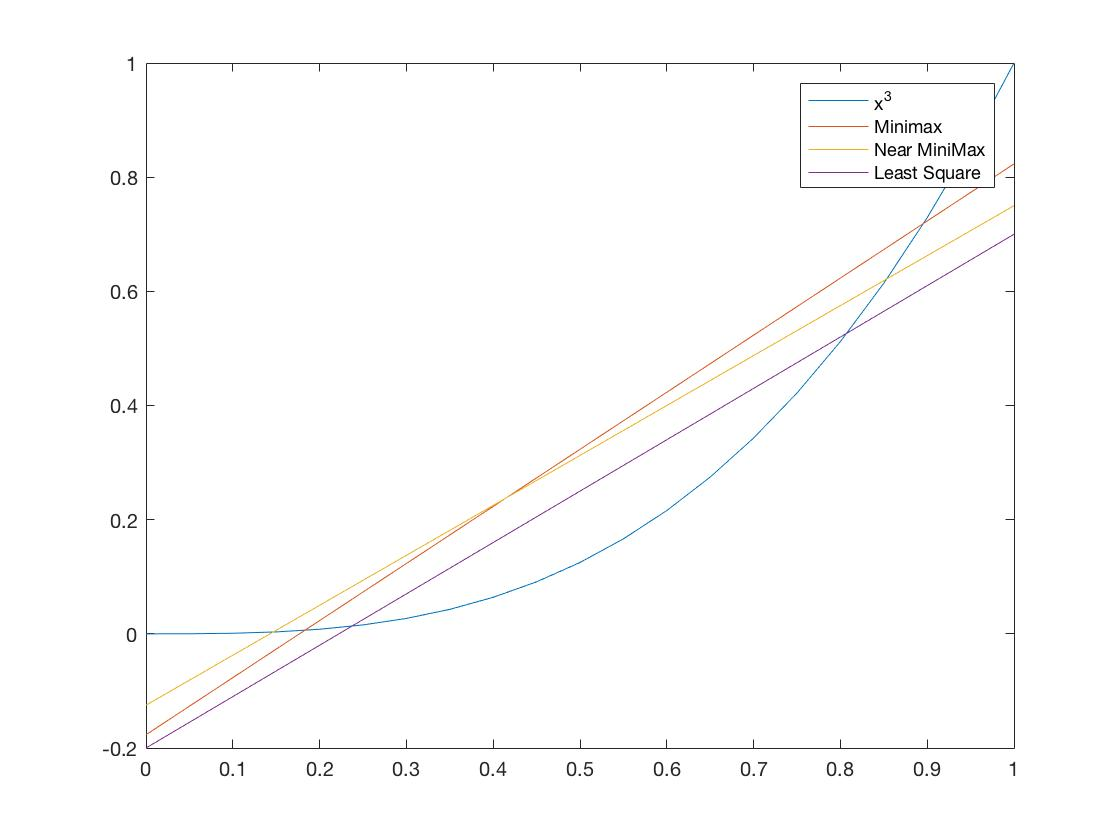
\includegraphics[width=\textwidth]{7a}

\paragraph{b. } Approximations on [-1,1]

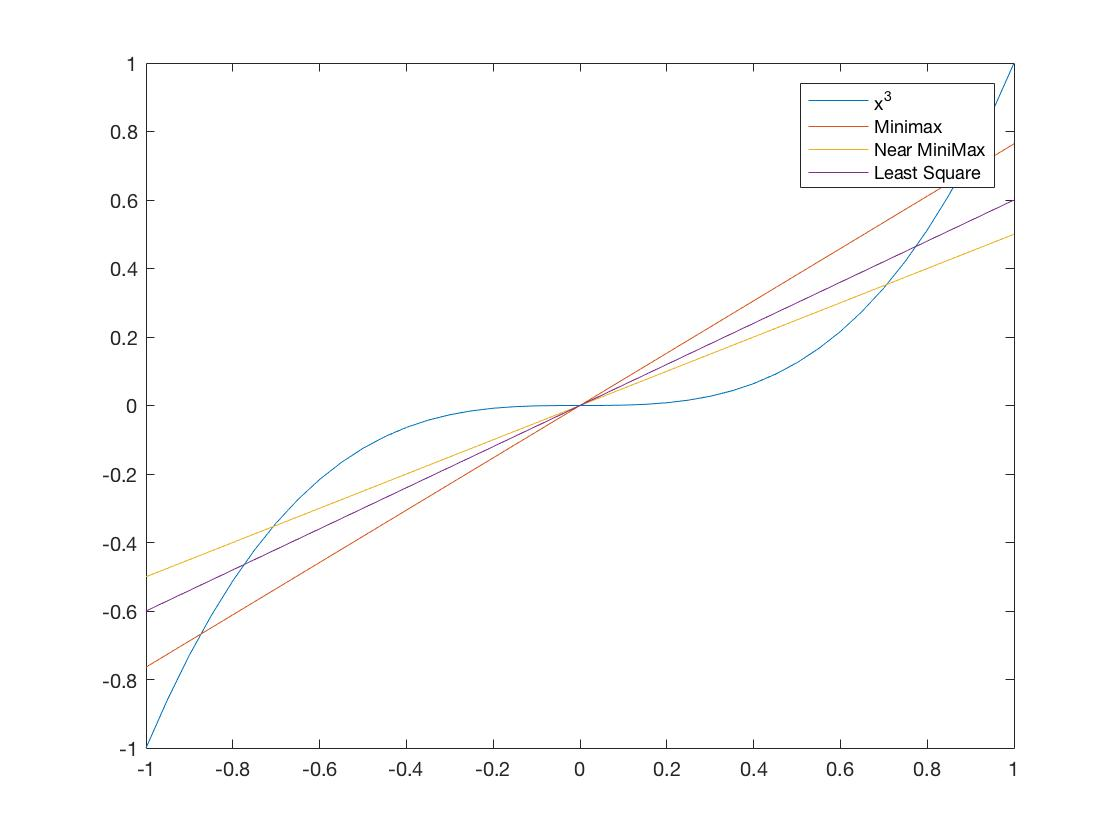
\includegraphics[width=\textwidth]{7b}




\end{document}
